\section{曲线积分}

曲线积分是对向量场沿着曲线进行积分的数学工具,用于描述向量场沿着曲线的积分值. 曲线积分可以分为第一类曲线积分和第二类曲线积分.

\subsection{两类曲线积分}

\subsubsection{第一类曲线积分的计算}

\begin{definition}[对弧长的曲线积分 (第一类曲线积分)]
    $\displaystyle\int_L f(x,y)\dd s=\lim_{\lambda\to0}\sum_{i=1}^{n}f(\xi_i,\eta_i)\Delta s_i$,如果函数 $f(x,y)$ 在曲线 $L$ 上连续,
    则 $f(x,y)$ 在曲线 $L$ 上对弧长的曲线积分 $\displaystyle\int_L f(x,y)\dd s$ 一定存在.\\
    上述概念可以推广到空间,如果 $f(x,y,z)$ 是定义在空间中分段光滑曲线 $L$ 上的有界函数,则函数 $f(x,y,z)$ 在曲线 $L$ 上对弧长的曲线积分是
    $$\int_Lf(x,y,z)\dd s=\lim_{\lambda\to0}\sum_{i=1}^{n}f(\xi_i,\eta_i,\zeta_i)\Delta s_i.$$
\end{definition}

\begin{theorem}
    第一类曲线积分有如下基本性质:
    \begin{enumerate}[label=(\arabic{*})]
        \item $\displaystyle\int_L [f_1(x,y)\pm f_2(x,y)]\dd s=\int_L f_1(x,y)\dd s+\int_L f_2(x,y)\dd s+$;
        \item $\displaystyle\int_L kf(x,y)\dd s=k\int_L f(x,y)\dd s$,其中 $k$ 为常数;
        \item 若 $L=L_1+L_2$,且 $L_1$ 与 $L_2$ 无公共点,则 $$\int_Lf(x,y)\dd s=\int_{L_1}f(x,y)\dd s+\int_{L_2}f(x,y)\dd s. $$
    \end{enumerate}
\end{theorem}

\begin{theorem}[轴对称性]
    若积分弧段 $L$ 关于 $y$ 轴对称,则
    $$I=\begin{cases}
            2\displaystyle \int_{L_1}f(x,y)\dd s, & f(x,y)=f(-x,y)  \\
            0,                                    & f(x,y)=-f(-x,y)
        \end{cases}$$
    其中 $L_1=\qty{(x,y)\mid (x,y)\in L,x\geqslant 0}$.\\
    若积分弧段 $L$ 关于 $x$ 轴对称,则
    $$I=\begin{cases}
            2\displaystyle\int_{L_2}f(x,y)\dd s, & f(x,y)=f(x,-y)  \\
            0,                                   & f(x,y)=-f(x,-y)
        \end{cases}$$
    其中 $L_2=\qty{(x,y)\mid (x,y)\in L,y\geqslant 0}$.
\end{theorem}

\begin{theorem}[轮换对称性]
    若把 $x$ 与 $y$ 对调后,$L$ 不变,则 $$\int_L f(x,y)\dd s=\int_Lf(y,x)\dd s.$$
\end{theorem}

\begin{example}
    设曲线 $L:\begin{cases}
            x^2+y^2+z^2=a^2 \\
            x+y+z=0
        \end{cases}$ 求 $\displaystyle\oint_L\qty(x^2+2y^2+z)\dd s.$
\end{example}
\begin{solution}
    有轮换对称性 $\displaystyle\oint_Lx^2\dd s=\oint_Ly^2\dd s=\oint_Lz^2\dd s=\dfrac{1}{3}\oint_L\qty(x^2+y^2+z^2)\dd s,~\oint_Lx\dd s=\oint_Ly\dd s=\oint_Lz\dd s=\dfrac{1}{3}\oint_L(x+y+z)\dd s$,因此
    $$\oint_L\qty(x^2+2y^2+z)\dd s=\oint_L\qty(x^2+y^2+z^2)\dd s+\dfrac{1}{3}\oint_L(x+y+z)\dd s=a^2\oint_L\dd s+0=2\pi a^3.$$
\end{solution}

\begin{example}
    设 $L:\begin{cases}
            (x-1)^2+(y-1)^2+(z-1)^2=3 \\
            x+y+z=3
        \end{cases}$ 求 $\displaystyle\oint_L\qty(x^2+y^2+z^2)\dd s.$
\end{example}
\begin{solution}
    将球心平移到坐标原点,即 $\begin{cases}
            X=x-1 \\
            Y=y-1 \\
            Z=z-1
        \end{cases}$ 那么 $L':\begin{cases}
            X^2+Y^2+Z^2=3 \\
            X+Y+Z=0
        \end{cases}$ 因此
    \begin{flalign*}
        \oint_L\qty(x^2+y^2+z^2)\dd s & =\oint_{L'}\qty[(X+1)^2+(Y+1)^2+(Z+1)^2]\dd s                                                              \\
                                      & =\oint_{L'}\qty(X^2+Y^2+Z^2)\dd s+2\oint_{L'}(X+Y+Z)\dd s+3\oint_{L'}\dd s=6\oint_{L'}\dd s=12\sqrt{3}\pi.
    \end{flalign*}
\end{solution}

\begin{theorem}[第一类曲线积分化为定积分]
    \begin{enumerate}[label=(\arabic{*})]
        \item 直角坐标形式\\
              平面曲线 $ L $ 由直角坐标 $ y=y(x), a \leqslant x \leqslant b $ 给出,则:
              $$\int_{L} f(x, y) \dd  s=\int_{a}^{b} f(x, y(x)) \sqrt{1+\left[y^{\prime}(x)\right]^{2}} \dd  x .$$
        \item 参数方程形式\\
              平面曲线 $ L $ 由参数方程 $ \begin{cases}
                      x=\varphi(t) \\ y=\psi(t)\\\alpha \leqslant t \leqslant \beta
                  \end{cases} $ 给出,则:
              $$\int_{L} f(x, y) \dd  s=\int_{\alpha}^{\beta} f(\varphi(t), \psi(t)) \sqrt{\left[\varphi^{\prime}(t)\right]^{2}+\left[\psi^{\prime}(t)\right]^{2}} \dd  t .$$
        \item 极坐标形式\\
              平面曲线 $ L $ 由极坐标 $ r=r(\theta), \alpha \leqslant \theta \leqslant \beta $ 给出,则:
              $$\int_{L} f(x, y) \dd  s=\int_{\alpha}^{\beta} f(r(\theta) \cos \theta, r(\theta) \sin \theta) \sqrt{[r(\theta)]^{2}+\left[r^{\prime}(\theta)\right]^{2}} \dd  \theta .$$
        \item 空间曲线 $\Gamma $ 由参数方程 $\begin{cases}
                      x=\varphi(t) \\ y=\psi(t)\\ z=\omega(t)\\\alpha \leqslant t \leqslant \beta
                  \end{cases}$ 给出,则:
              $$\int_{\Gamma} f(x, y, z) \dd  s =\int_{\alpha}^{\beta} f(\varphi(t), \psi(t), \omega(t))\sqrt{\left[\varphi^{\prime}(t)\right]^{2}+\left[\psi^{\prime}(t)\right]^{2}+\left[\omega^{\prime}(t)\right]^{2}} \dd  t .$$
    \end{enumerate}
\end{theorem}

\begin{example}
    设 $L$ 是由点 $O(0,0),~A(2,0)$ 及 $B(2,2)$ 所围成的三角形的周界,计算曲线积分 $\displaystyle\oint_L(x+y)\dd s.$
\end{example}
\begin{solution}
    $OA: y=0,~x\in[0,2],~\displaystyle\int_{\overline{OA}}(x+y)\dd s=\int_{0}^{2}x\dd x=2$; $\displaystyle AB: x=2,~y\in[0,2],~\int_{\overline{AB}}(x+y)\dd s=\int_{0}^{2}(2+y)\dd y=6$;
    $$OB: y=x,~x\in[0,2],~\int_{\overline{OB}}(x+y)\dd s=\int_{0}^{2}(2x)\sqrt{1+y'^2}\dd x=4\sqrt{2}$$
    因此 $\displaystyle\oint_L (x+y)\dd s=8+4\sqrt{2}.$
\end{solution}

\begin{example}[2009 数一]
    已知曲线 $L:y=x^2~ \qty(0\leqslant x\leqslant \sqrt{2})$,求 $\displaystyle\int_Lx\dd s.$
\end{example}
\begin{solution}
    $\dd s=\sqrt{1+y'^2}\dd x=\sqrt{1+4x^2}\dd x$,于是
    $$\int_L x\dd s=\int_{0}^{\sqrt{2}}x\sqrt{1+4x^2}\dd x=\eval{\dfrac{1}{8}\cdot\dfrac{2}{3}\qty(1+4x^2)^{\frac{3}{2}}}_{0}^{\sqrt{2}}=\dfrac{13}{6}.$$
\end{solution}

\begin{example}
    设 $\Gamma:\begin{cases}
            x^2+y^2+z^2=a^2 \\ x+y+z=0
        \end{cases}$ 求曲线积分 $\displaystyle\int_\Gamma (x+y)^2\dd s.$
\end{example}
\begin{solution}
    \textbf{法一: }由 $x+y=-z$,于是 $\displaystyle\int_\Gamma(x+y)^2\dd s=\int_\Gamma z^2\dd s$,
    由轮换对称性知 $$\int_\Gamma x^2\dd s=\int_\Gamma y^2\dd s=\int_\Gamma z^2\dd s=\dfrac{1}{3}\qty(x^2+y^2+z^2)\dd s$$
    又 $x^2+y^2+z^2=a^2$,于是 $$\displaystyle\int_\Gamma (x+y)^2\dd s=\dfrac{1}{3}\int_\Gamma \qty(x^2+y^2+z^2)\dd s=\dfrac{a^2}{3}\int_\Gamma \dd s=\dfrac{2\pi}{3}a^3.$$
    \textbf{法二: }由 $z=-(x+y)$,代入 $x^2+y^2+z^2=a^2$,得 $x^2+y^2+xy=\dfrac{a^2A}{2}$,故由旋转变换
    $$x=\dfrac{\sqrt{2}}{2}(X+Y),~y=\dfrac{\sqrt{2}}{2}(X-Y)$$
    将其转换为 $3X^2+Y^2=a^2$,并令 $X=\dfrac{a}{\sqrt{3}}\cos t,Y=a\sin t,0\leqslant t\leqslant 2\pi$,
    可得 $\Gamma$ 的参数方程为 $$\begin{cases}
            x=\dfrac{\sqrt{2} }{2} \qty(\dfrac{a}{\sqrt 3}\cos t-a\sin t ) \\[6pt]
            y=\dfrac{\sqrt 2}{2}\qty(\dfrac{a}{\sqrt 3}\cos t+a\sin t )    \\[6pt]
            z=-\dfrac{\sqrt 6}{3}a\cos t                                   \\[6pt]
            0\leqslant  t\leqslant  2\pi
        \end{cases}$$
    又 $\dd s=\sqrt{\qty[x'(t)]^2+\qty[y'(t)]^2+\qty[z'(t)]^2}\dd t=a\dd t$,于是
    \begin{flalign*}
        I=\int_{0}^{2\pi}(x(t)+y(t))^2\sqrt{\qty[x'(t)]^2+\qty[y'(t)]^2+\qty[z'(t)]^2}\dd t=\int_{0}^{2\pi}\qty(\dfrac{\sqrt{6}}{3}a\cos t)^2\cdot a\dd t=\dfrac{2}{3}a^3\int_{0}^{2\pi}\cos^2t\dd t=\dfrac{2}{3}\pi a^3.
    \end{flalign*}
\end{solution}

\subsubsection{第二类曲线积分的计算}

\begin{definition}[对坐标的曲线积分 (第二类曲线积分)]
    \begin{flalign*}
        \int_L P(x,y)\dd x & =\lim_{\lambda\to0}\sum_{i=1}^{n}P(\xi_i,\eta_i)\Delta x_i \\
        \int_L Q(x,y)\dd y & =\lim_{\lambda\to0}\sum_{i=1}^{n}Q(\xi_i,\eta_i)\Delta y_i
    \end{flalign*}
    如果函数 $P(x,y),~Q(x,y)$ 在有向曲线 $L$ 上连续时,上述积分都存在. 类似地,在空间中有向曲线 $\Gamma$ 上对坐标 $x,y,z$ 的曲线积分
    \begin{flalign*}
        \int_L P(x,y,z)\dd x & =\lim_{\lambda\to0}\sum_{i=1}^{n}P(\xi_i,\eta_i,\zeta_i)\Delta x_i  \\
        \int_L Q(x,y,z)\dd y & =\lim_{\lambda\to0}\sum_{i=1}^{n}Q(\xi_i,\eta_i,\zeta_i)\Delta y_i  \\
        \int_L R(x,y,z)\dd z & =\lim_{\lambda\to0}\sum_{i=1}^{n}R(\xi_i,\eta_i,\zeta_i)\Delta z_i.
    \end{flalign*}
\end{definition}

\begin{theorem}
    $\displaystyle \int_{\widehat{AB} }P\dd x+Q\dd y=-\int_{\widehat{BA} }P\dd x+Q\dd y.$
\end{theorem}

\begin{theorem}[第二类曲线积分化为定积分]
    \begin{enumerate}[label=(\arabic{*})]
        \item 设函数 $P(x,y),~Q(x,y)$ 在有向曲线 $L$ 上连续,$L$ 的参数方程为 $\begin{cases}
                      x=x(t) \\ y=y(t)
                  \end{cases}(\alpha\leqslant t\beta)$,且 $x'(t),~y'(t)$ 连续,而 $t=\alpha$ 时对应于起点 $A$,$t=\beta$ 时对应于终点 $B$,则
              \begin{flalign*}
                  \int_{\widehat{AB} }P(x,y)\dd x & =\int_{\alpha}^{\beta}P[x(t),y(t)]x'(t)\dd t \\
                  \int_{\widehat{AB} }Q(x,y)\dd y & =\int_{\alpha}^{\beta}Q[x(t),y(t)]y'(t)\dd t
              \end{flalign*}
        \item 如果曲线 $L$ 由方程 $y=y(x)~~(a\leqslant x\leqslant b)$ 给出,曲线 $L$ 的起点 $A$ 的横坐标为 $x=a$,终点 $B$ 的横坐标为 $x=b$,
              函数 $y(x)$ 具有连续的一阶导数,则
              \begin{flalign*}
                  \int_{\widehat{AB} }P(x,y)\dd x & =\int_{a}^{b}P[x,y(x)]\dd x      \\
                  \int_{\widehat{AB} }Q(x,y)\dd y & =\int_{a}^{b}Q[x,y(x)]y'(x)\dd x
              \end{flalign*}
        \item 如果曲线 $L$ 由方程 $x=x(y)~~(c\leqslant y\leqslant d)$ 给出,曲线 $L$ 的起点 $A$ 的横坐标为 $y=c$,终点 $B$ 的横坐标为 $y=d$,
              函数 $x(y)$ 具有连续的一阶导数,则
              \begin{flalign*}
                  \int_{\widehat{AB} }P(x,y)\dd x & =\int_{c}^{d}P[x(y),y]x'(y)\dd y \\
                  \int_{\widehat{AB} }Q(x,y)\dd y & =\int_{c}^{d}Q[x(y),y]\dd y
              \end{flalign*}
        \item 对于空间曲线积分,如果函数 $P(x,y,z),~Q(x,y,z),~R(x,y,z)$ 在有向曲线 $\Gamma$ 上连续,$\Gamma$ 的参数方程为 $\begin{cases}
                      x=x(t) \\ y=y(t) \\ z=z(t)
                  \end{cases}(\alpha \leqslant t\leqslant \beta)$,且 $x'(t),~y'(t),~z'(t)$ 连续,而 $t=\alpha$ 时对应于起点 $A$,$t=\beta$ 时对应于终点 $B$,则
              \begin{flalign*}
                  \int_{\widehat{AB} }P(x,y,z)\dd x & =\int_{\alpha}^{\beta}P[x(t),y(t),z(t)]x'(t)\dd t  \\
                  \int_{\widehat{AB} }Q(x,y,z)\dd y & =\int_{\alpha}^{\beta}Q[x(t),y(t),z(t)]y'(t)\dd t  \\
                  \int_{\widehat{AB} }R(x,y,z)\dd z & =\int_{\alpha}^{\beta}R[x(t),y(t),z(t)]z'(t)\dd t.
              \end{flalign*}
    \end{enumerate}
\end{theorem}

\begin{example}[2004 数一]
    设 $L$ 为正向圆周 $x^2+y^2=2$ 在第一象限中的部分,求曲线积分 $\displaystyle\int_Lx\dd y-2y\dd x.$
\end{example}
\begin{solution}
    正向圆周在第一象限内可表示为 $\begin{cases}
            x=\sqrt{2}\cos\theta \\y=\sqrt{2}\sin\theta\\\theta\in\qty[0,\dfrac{\pi}{2}]
        \end{cases}$
    于是 $$\int_Lx\dd y-2y\dd x=\int_{0}^{\frac{\pi}{2}}\qty(2+2\sin^2\theta)\dd \theta=2\int_{0}^{\frac{\pi}{2}}\dd \theta+2\int_{0}^{\frac{\pi}{2}}\sin^2\theta\dd \theta=\dfrac{3\pi}{2}.$$
\end{solution}

\begin{example}
    设 $L$ 是从点 $A(-1,1)$ 沿曲线 $x^2+y^2=-2y~~(y\geqslant -1)$ 到点 $B(-1,-1)$ 的有向线段,$f(x)$ 是连续函数,计算
    $$I=\int_Lx[f(x)+1]\dd y-\dfrac{y^2[f(x)+1]+2yf(x)}{\sqrt{1-x^2}}\dd x.$$
    \begin{minipage}[b]{0.29\linewidth}
        \begin{figure}[H]
            \centering
            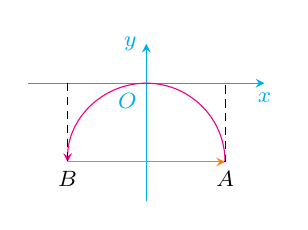
\begin{tikzpicture}[->,samples=100,>=stealth,font=\footnotesize]
                \draw[->,cyan](-1.5,0)--(0,0)node[below left]{$O$}--(1.5,0)node[below]{$x$};
                \draw[->,cyan](0,-1.5)--(0,0.5)node[left]{$y$};
                \draw[magenta] (1,-1) arc (0:180:1);
                \draw[densely dashed,-,black] (-1,0)--(-1,-1)node[below]{$B$}--(1,-1)node[below]{$A$}--(1,0);
                \draw[orange] (-1,-1)--(1,-1);
            \end{tikzpicture}
            \caption{}
        \end{figure}
    \end{minipage}\hfill
    \begin{minipage}[b]{0.7\linewidth}
        \begin{errorSolution}
            补一有向线段 $\overrightarrow{BA}$,然后用 Green 公式计算,\\
            令 $P=-\dfrac{y^2[f(x)+1]+2yf(x)}{\sqrt{1-x^2}},~Q=x[f(x)+1]$,那么 $\displaystyle\pdv{Q}{x}-\pdv{P}{y}=\cdots$.\\
            \textbf{错因: }这道题考查了第二型曲线积分的计算,注意到题目只说 $f$ 连续,并没有说\textbf{可导},所以不能用 Green 公式,只能用基本方法将 $I$ 化为定积分来计算.\\
        \end{errorSolution}
    \end{minipage}
\end{example}
\begin{solution}
    令 $x=\cos t,y=\sin t-1,~(0\leqslant t\leqslant \pi)$ 代入 $I$ 并化简,有
    \begin{flalign*}
        I & =\int_{0}^{\pi}\cos t[f(\cos t)+1]\cos t\dd t+\dfrac{(\sin t-1)^2[f(\cos t)+1]+2(\sin t-1)f(\cos t)}{\sin t}\sin t\dd t \\
          & =\int_{0}^{\pi}\qty{\cos^2t[f(\cos t)+1]+(\sin t-1)[f(\cos t)+1]+(2\sin t-2)f(\cos t)}\dd t                             \\
          & =2\int_{0}^{\pi}(1-\sin t)\dd t=\eval{2(t+\cos t)}_{0}^{\pi}=2\pi-4.
    \end{flalign*}
\end{solution}

\subsubsection{方向导数与两类曲线积分的联系}

\begin{example}
    设 $u(x,y)$ 于圆盘 $D=\qty{(x,y):x^2+y^2\leqslant \dfrac{\pi}{2}}$ 内有二阶连续的偏导数,并且满足:
    $$\pdv[2]{u}{x}+\pdv[2]{u}{y}=\qty(x^2+y^2)\sin^6\qty(x^2+y^2)$$
    记 $D$ 的正向边界曲线为 $\partial D$,$\partial D$ 的外法线向量为 $\va*{n}$,求 $\displaystyle \oint_{\partial D}\pdv{u}{\va*{n}}\dd s.$
\end{example}
\begin{solution}
    设 $\va*{T}=(\cos\alpha,\cos\beta)$ 对应的正向切线的单位向量,则单位向量为 $\va*{n}=(\cos\alpha,-\cos\beta)$,由题设可知 $u(x,y)$ 可微,
    故由方向导数计算公式和两类曲线积分之间的关系,得
    $$I=\oint_{\partial D}\pdv{u}{\va*{n}}\dd s=\oint_{\partial D}\qty(\pdv{u}{x}\cos \beta-\pdv{u}{y}\cos \alpha)\dd s=\oint_{\partial D}\pdv{u}{x}\dd y-\pdv{u}{y}\dd x$$
    于是由 Green 公式和二重积分的极坐标计算公式,得
    \begin{flalign*}
        I & =\iint\limits_D\qty(\pdv[2]{u}{x}+\pdv[2]{u}{y})\dd x\dd y=\iint\limits_D\qty(x^2+y^2)\sin^6\qty(x^2+y^2)\dd x\dd y=\int_{0}^{2\pi}\dd \theta\int_{0}^{\sqrt{\frac{\pi}{2}}}r^2\sin^6r^2\dd r=\pi\int_{0}^{\frac{\pi}{2}}u\sin^6u\dd u
    \end{flalign*}
    又因为 $\sin^nx=\begin{cases}
            \displaystyle \dfrac{1}{(2\i)^{n-1}}\sum_{k=0}^{\frac{n-1}{2}}(-1)^k\C_n^k\cos((n-2k)x) \\
            \displaystyle \dfrac{2}{(2\i)^n}\qty[\sum_{k=0}^{\frac{n}{2}-1}(-1)^k\C_n^k\cos((n-2k)x)+\dfrac{(-1)^{\frac{n}{2}}}{2}\C_n^{\frac{n}{2}}]
        \end{cases}\Rightarrow \sin^6x=-\dfrac{1}{8}\cos^32x+\dfrac{3}{16}\cos 4x-\dfrac{3}{8}\cos 2x+\dfrac{5}{16}$,由分部积分公式
    $$\int u\cos nu\dd u=\dfrac{\cos nu}{n^2}+\dfrac{u\sin nu}{n}+C$$
    分别取 $n=2,4,6$,得 $\displaystyle I=\pi\qty(\dfrac{17}{72}+\dfrac{5\pi^2}{128}).$
\end{solution}

\subsection{Green 公式}

\begin{theorem}[Green 公式]
    Green 公式给出了平面上有限条逐段光滑封闭曲线上的线积分与它们所包围区域上的二重积分的关系:
    $$\oint_{L^+}P\dd x+Q\dd y=\iint\limits_D\left(\frac{\partial Q}{\partial x}-\frac{\partial P}{\partial y}\right)\dd x\dd y$$
    这里 $L^+$ 表示沿 $L$ 的正向取积分. 正向指前进时  保持在左边的方向,当 $D$ 为单连通区域时,
    即是逆时针方向;当 $D$ 为多联通区域时,外边界为逆时针方向,内边界为顺时针方向. $P,Q$ 要求
    在区域 $D$ 内直到边界 $L$ 上连续,并且连续偏导数. 由此可得 $D$ 的面积公式为:
    $$S=\iint\limits_D\dd x\dd y=\oint_{L^+}x\dd y=-\oint_{L^-}y\dd x=\frac{1}{2}\int_Lx\dd y-y\dd x.$$
\end{theorem}

\subsubsection{计算封闭曲线上的线积分}

\begin{example}
    已知 $L$ 是区域 $D:\dfrac{x}{2}\leqslant y\leqslant 2x,~1\leqslant xy\leqslant 2$ 的正向边界曲线,求
    $$\displaystyle\oint_L\mathrm{e}^{x^2y^2}\qty[\qty(y-\dfrac{1}{x})\dd x+\qty(x+\dfrac{1}{y})\dd y].$$
\end{example}
\begin{solution}
    令 $u=\dfrac{y}{x},~v=xy$,那么 $x=\sqrt{\dfrac{v}{u}},~y=\sqrt{uv}$,$\dd u=\dd \qty(\dfrac{y}{x})=\dfrac{x\dd y-y\dd x}{x^2}$,$\dd v=\dd (xy)=y\dd x+x\dd y$,
    $L'$ 是区域 $D':\dfrac{1}{2}\leqslant u\leqslant 2,~1\leqslant v\leqslant 2$ 的正向边界曲线,于是
    \begin{flalign*}
        I & =\oint_L\mathrm{e}^{x^2y^2}\qty[\qty(y-\dfrac{1}{x})\dd x+\qty(x+\dfrac{1}{y})\dd y]=\oint_L\mathrm{e}^{x^2y^2}\qty(y\dd x+x\dd y+\dfrac{x}{y}\cdot\dfrac{x\dd y-y\dd x}{x^2})                                             \\
          & =\oint_{L'}\mathrm{e}^{v^2}\qty(\dd v+\dfrac{1}{u}\dd u)=\iint\limits_{D'}\dfrac{2v\mathrm{e}^{v^2}}{u}\dd u\dd v=\int_{\frac{1}{2}}^2\dd u\int_1^2\dfrac{2v\mathrm{e}^{v^2}}{u}\dd v=2\ln 2\qty(\mathrm{e}^4-\mathrm{e}).
    \end{flalign*}
\end{solution}

\begin{example}
    设 $\Gamma $ 为 $x^2+y^2=2x(y\geqslant 0)$ 上从 $O(0,0)$ 到 $A(2,0)$ 的一段弧,连续函数 $f(x)$ 满足
    $$f(x)=x^2+\int_\Gamma y[f(x)+\mathrm{e}^x]\dd x+\qty(\mathrm{e}^x+xy^2)\dd y$$
    求 $f(x).$
\end{example}
\begin{solution}
    设 $\displaystyle \int_\Gamma y[f(x)+\mathrm{e}^x]\dd x+\qty(\mathrm{e}^x+xy^2)\dd y=a$,那么
    \begin{flalign*}
        a & =\qty(\int_{\Gamma+\overline{AO}}-\int_{\overline{AO}})y[f(x)+\mathrm{e}^x]\dd x+\qty(\mathrm{e}^x+xy^2)\dd y=-\iint\limits_{D}\qty[\pdv{x}\qty(\mathrm{e}^x-xy^2)-\pdv{y}\qty(y(f(x)+\mathrm{e}^x))]\dd x\dd y            \\
          & =-\iint\limits_D\qty(\mathrm{e}^x-y^2-x^2-a-\mathrm{e}^x)\dd x\dd y=\iint\limits_D\qty(x^2+y^2)\dd x\dd y+a\iint\limits_D\dd x\dd y=\int_0^{\frac{\pi}{2}}\dd \theta \int_0^{2\cos\theta }\rho^3\dd \rho +\dfrac{\pi a}{2} \\
          & =4\int_0^{\frac{\pi}{2}}\cos^4\theta\dd \theta +\dfrac{\pi a}{2}=\dfrac{3}{4}\pi+\dfrac{\pi a}{2}\Rightarrow a=\dfrac{3\pi}{2(2-\pi)}\Rightarrow f(x)=x^2+\dfrac{3\pi}{2(2-\pi)}.
    \end{flalign*}
\end{solution}

\begin{example}
    计算积分 $\displaystyle I=\oint_{L^+}\frac{x\dd y-y\dd x}{[(\alpha x+\beta y)^2+(\gamma x+\delta y)^2]^\alpha}~~(\alpha\delta-\beta\gamma\not=0)$,其中 $L^+$ 为椭圆 $(\alpha x+\beta y)^2+(\gamma x+\delta y)^2=1$,取逆时针方向.
\end{example}
\begin{solution}
    $L$ 上 $(\alpha x+\beta y)^2+(\gamma x+\delta y)^2=1$,因此
    $$\displaystyle I=\oint_{L^+}x\dd y-y\dd x=2\iint\limits_{(\alpha x+\beta y)^2+(\gamma x+\delta y)^2\leqslant  1}\dd x\dd y$$
    令 $u=\alpha x+\beta y,~v=\gamma x+\delta y$,作变换,有 $\displaystyle I=2\iint\limits_{u^2+v^2\leqslant  1}|J|\dd x\dd y$,其中
    $$J=\frac{\partial (x,y)}{\partial (u,v)}=\frac{1}{\alpha\delta-\beta\gamma}$$
    因此 $\displaystyle I=\frac{2}{|\alpha\delta-\beta\gamma|}\iint\limits_{u^2+v^2\leqslant  1}\dd u\dd v=\frac{2\pi}{|\alpha\delta-\beta\gamma|}.$
\end{solution}

\subsubsection{含有奇点形式}

\begin{example}
    设 $D=\qty{(x,y)\mid x^2+y^2\leqslant 4}$,$\partial D$ 为 $D$ 的正向边界,求
    $$I=\int_{\partial D}\dfrac{\qty(x\e^{x^2+4y^2}+y)\dd x+\qty(4y\e^{x^2+4y^2}-x)\dd y}{x^2+4y^2}.$$
\end{example}
\begin{solution}
    设 $l:x^2+4y^2=\varepsilon^2$,$\varepsilon$ 充分小且大于 0,取顺时针,如图 \ref{varepverylll} 所示,\\
    \begin{minipage}{0.29\linewidth}
        \begin{figure}[H]
            \centering
            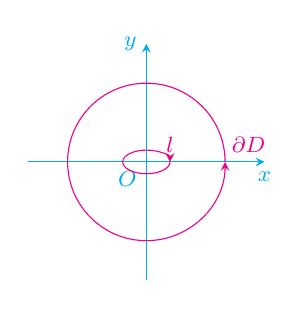
\begin{tikzpicture}[->,samples=100,>=stealth,font=\footnotesize]
                \draw[->,cyan](-1.5,0)--(0,0)node[below left]{$O$}--(1.5,0)node[below]{$x$};
                \draw[->,cyan](0,-1.5)--(0,1.5)node[left]{$y$};
                \draw[magenta] (1,0) arc (0:360:1)node[above]{$~~~~~~\partial D$};
                \draw[magenta,xscale=2] (0.15,0) arc (360:0:0.15)node[above]{$l$};
            \end{tikzpicture}
            \caption{}
            \label{varepverylll}
        \end{figure}
    \end{minipage}\hfill
    \begin{minipage}{0.7\linewidth}
        则有 $$\int_{\partial D}=\int_{\partial D+l-l}=\int_{\partial D+l}+\int_{l^-}:=I_1+I_2$$
        设 $P=\dfrac{x\e^{x^2+4y^2}+y}{x^2+4y^2},~Q=\dfrac{4y\e^{x^2+4y^2}-x}{x^2+4y^2}$,那么
        $$\pdv{Q}{x}=\dfrac{8xy\e^{x^2+4y^2}\qty(x^2+4y^2-1)+x^2-4y^2}{\qty(x^2+4y^2)^2}=\pdv{P}{y}$$
        因此 $\displaystyle I_1=\iint\limits_D\qty(\pdv{Q}{x}-\pdv{P}{y})\dd x\dd y=0$,下求 $I_2$,
    \end{minipage}
    \begin{flalign*}
        I_2 & =\dfrac{1}{\varepsilon^2}\int_{l^-}\underbrace{\qty(x\e^{x^2+4y^2}+y)}_{P_1}\dd x+\underbrace{\qty(4y\e^{x^2+4y^2}-x)}_{Q_1}\dd y=\dfrac{1}{\varepsilon^2}\iint\limits_{D_{\varepsilon}}\qty(\pdv{Q_1}{x}-\pdv{P_1}{y})\dd x\dd y \\
            & =\dfrac{-2}{\varepsilon^2}\iint\limits_{x^2+4y^2\leqslant \varepsilon^2}\dd x\dd y=\dfrac{-2}{\varepsilon^2}\cdot\pi\cdot\varepsilon\cdot\dfrac{\varepsilon}{2}=-\pi
    \end{flalign*}
    故 $I=0-\pi=\pi.$
\end{solution}

\begin{example}
    计算 $\displaystyle\oint_{C^+}\frac{x\dd y-y\dd x}{4x^2+y^2}$,$C$ 为以 $(1,0)$ 为圆心,以 $R$ 为半径的圆周 ($R\not=1$),设 $C^+$ 表示其上的方向为逆时针方向.
\end{example}
\begin{solution}
    当 $R<1$ 时,满足 Green 公式的条件,则 $$\frac{\partial }{\partial x}\left(\frac{x}{4x^2+y^2}\right)=\frac{y^2-4x^2}{(4x^2+y^2)^2}=\frac{\partial }{\partial y}\left(\frac{-y}{4x^2+y^2}\right)$$
    所以 $\displaystyle\oint_{C^+}\frac{x\dd y-y\dd x}{4x^2+y^2}=0~~(x,y\not=0)$;\\
    当 $R>1$ 时,取 $\varepsilon>0$ 充分小,使得 $\Gamma_\varepsilon:~4x^2+y^2=\varepsilon^2$,且 $\Gamma_\varepsilon^+$ 表示其上的方向为顺时针方向,
    记 $C$ 与 $\Gamma$ 所围成区域为 $D$,则 $\displaystyle\oint_{C^++\Gamma_\varepsilon^+}\frac{x\dd y-y\dd x}{4x^2+y^2}=0$,
    那么 $$\oint_{C^+}\frac{x\dd y-y\dd x}{4x^2+y^2}=\oint_{\Gamma_\varepsilon^-}\frac{x\dd y-y\dd x}{4x^2+y^2}=\frac{1}{\varepsilon^2}\oint_{\Gamma_\varepsilon^-}x\dd y-y\dd x=\frac{1}{\varepsilon^2}\cdot \pi\varepsilon^2=\pi.$$
\end{solution}

\begin{example}
    设 $f(x,y)$ 单位圆上有连续的偏导数,且在边界上取值为零,求证: $$\displaystyle\lim_{\varepsilon\to 0^+}\iint\limits_D\dfrac{x\dfrac{\partial f}{\partial x}+y\dfrac{\partial f}{\partial y}}{x^2+y^2}\dd x\dd y=-2\pi f(0,0).$$ 其中 $D$ 为圆环域: $\varepsilon ^2\leqslant  x^2+y^2\leqslant  1.$
\end{example}
\begin{proof}[{\songti \textbf{证}}]
    记 $\displaystyle L_1:~x^2+y^2=1$ (逆时针方向),$L_2:~x^2+y^2=\varepsilon ^2$ (顺时针方向),
    \begin{flalign*}
        \iint\limits_D\dfrac{x\dfrac{\partial f}{\partial x}+y\dfrac{\partial f}{\partial y}}{x^2+y^2}\dd x\dd y & =\oint_{L_2}\dfrac{-yf(x,y)\dd x+xf(x,y)\dd y}{x^2+y^2}=\dfrac{1}{\varepsilon^2}\oint_{L_2}-yf(x,y)\dd x+xf(x,y)\dd y                                                                                 \\
                                                                                                                 & =\dfrac{1}{\varepsilon^2}\int_{2\pi}^0\left[(-\varepsilon\sin\theta)(-\varepsilon\sin\theta)+\epsilon\cos\theta\cdot\epsilon\cos\theta\right]f(\varepsilon\cos\theta,\varepsilon\sin\theta)\dd \theta \\
                                                                                                                 & =-\int_0^{2\pi}f(\varepsilon\cos\theta,\varepsilon\sin\theta)\dd \theta=-2\pi f(\varepsilon\cos\theta^*,\varepsilon\sin\theta^*)~~(\theta^*\in[0,2\pi])
    \end{flalign*}
    故 $\displaystyle\lim_{\varepsilon\to0^+}\iint\limits_D\dfrac{x\dfrac{\partial f}{\partial x}+y\dfrac{\partial f}{\partial y}}{x^2+y^2}\dd x\dd y=-2\pi f(0,0).$
\end{proof}

\subsubsection{外法向量形式}

\begin{example}
    设 $u(x,y)$ 于圆盘 $D:x^2+y^2\leqslant  \pi$ 内有二阶连续偏导数,且
    $$\displaystyle\frac{\partial ^2u}{\partial x^2}+\frac{\partial ^2u}{\partial y^2}=\mathrm{e}^{\pi-x^2-y^2}\sin\left(x^2+y^2\right)$$
    记 $D$ 的正向边界曲线为 $\partial D$,$\partial D$ 的外法线向量为 $\boldsymbol n$,求 $\displaystyle\oint_{\partial D}\frac{\partial u}{\partial \boldsymbol n}\dd s.$
\end{example}
\begin{solution}
    令 $\boldsymbol n=(\cos\alpha,\cos\beta)$,则 $\displaystyle \frac{\partial u}{\partial \boldsymbol n}=\frac{\partial u}{\partial x}\cos\alpha+\frac{\partial u}{\partial y}\cos\beta$,$\partial D$ 的单位切向量 $\boldsymbol \tau=(-\cos\beta,\cos\alpha)$,于是
    \begin{flalign*}
        \oint_{\partial D}\frac{\partial u}{\partial \boldsymbol n}\dd s & =\int_{\partial D}\left(\frac{\partial u}{\partial x}\cos\alpha+\frac{\partial u}{\partial y}\cos\beta\right)\dd s=\int_{\partial D}\frac{\partial u}{\partial x}\dd y-\frac{\partial u}{\partial y}\dd x=\iint\limits_D\left(\frac{\partial ^2u}{\partial x^2}+\frac{\partial ^2u}{\partial y^2}\right)\dd x\dd y \\
                                                                         & =\iint\limits_{D}\mathrm{e}^{\pi-x^2-y^2}\sin\left(x^2+y^2\right)\dd x\dd y
        =\int_0^{2\pi}\dd \theta\int_0^{\sqrt{\pi}}\rho\mathrm{e}^{\pi-\rho^2}\sin\left(\rho^2\right)\dd \rho                                                                                                                                                                                                                                                                                 \\
                                                                         & \xlongequal[]{t=\rho^2}\pi\int_0^\pi\mathrm{e}^{\pi-t}\sin t\dd t=\frac{\pi}{2}\left(\mathrm{e}^\pi+1\right).
    \end{flalign*}
\end{solution}
\begin{example}
    设函数 $u(x,y)$ 在区域 $D=\left\{(x,y)|x^2+y^2\leqslant \pi\right\}$ 上有二阶连续偏导数,且
    $$\frac{\partial^2u}{\partial x^2}+\frac{\partial ^2u}{\partial y^2}=\mathrm{e}^{\pi-x^2-y^2}\cdot\sin\left(x^2+y^2\right)$$
    记 $D$ 的正向边界曲线为 $L$,$L$ 的外法向量为 $\vec{n}$,求 $\displaystyle\oint_L\frac{\partial u}{\partial \vec{n}}\dd s.$
\end{example}
\begin{solution}
    因为$$ \oint_L\frac{\partial u}{\partial \vec{n}}\dd s=\iint\limits_D\left(\frac{\partial ^2u}{\partial x^2}+\frac{\partial ^2u}{\partial y^2}\right)\dd x\dd y$$
    所以
    \begin{flalign*}
        \oint_L\frac{\partial u}{\partial \vec{n}}\dd s =\iint\limits_D\mathrm{e}^{\pi-x^2-y^2}\cdot\sin\left(x^2+y^2\right)\dd x\dd y
        =\int_0^{2\pi}\dd \theta\int_0^{\sqrt{\pi}}\rho\mathrm{e}^{\pi-\rho^2}\sin\rho^2\dd \rho
        =\pi\int_0^\pi\mathrm{e}^{\pi-t}\sin t\dd t=\frac{\pi}{2}\left(\mathrm{e}^\pi+1\right)
    \end{flalign*}
\end{solution}

\subsubsection{积分与路径无关问题}

该部分内容可能需要结合第八章“微分方程”的知识,若不熟悉常见的微分方程求解,可暂缓阅读.

\begin{definition}[单连通与复连通区域]
    若平面区域 $ D $ 内任一闭曲线所围的部分都属于 $D$,则称 $ D $ 为\textit{平面单连通区域},否则称为\textit{复连通区域}. 通俗地讲,平面单连通区域就是不含有“洞”的区域.
\end{definition}

\begin{theorem}[路径无关]
    设函数 $ P(x, y), Q(x, y) $ 在区域 $ D $ 内具有一阶连续 偏导数,若对于 $ D $ 内的任意指定的两点  $A, B$  以及 $ D $ 内从点  $A$  到点 $ B$  的两条任意曲线 $ L_{1}, L_{2}$,等式
    $$\int_{L_{1}} P \dd  x+Q \dd  y=\int_{L_{2}} P \dd  x+Q \dd  y$$
    恒成立,则称曲线积分 $ \displaystyle\int_{L} P \dd  x+Q \dd  y $ 在 $ D $ 内与路径无关,否则称与路径有关.
    \index{路径无关}
\end{theorem}

设在单连通区域 $ D $ 内 $ P, Q $ 具有一阶连续偏导数,则下述 6 个说法等价
\begin{enumerate}[label=(\arabic{*})]
    \item $\displaystyle\int_{L} P(x, y) \dd  x+Q(x, y) \dd  y $ 在 $ D $ 内与路径无关;
    \item $\displaystyle \oint_{L} P(x, y) \dd  x+Q(x, y) \dd  y=0 $
          其中 $ L $ 是区域 $ D $ 内任意分段光滑闭曲线.
    \item $P \dd  x+Q \dd  y=d u(x, y)$;
    \item $\displaystyle\frac{\partial Q}{\partial x}=\frac{\partial P}{\partial y}, \forall(x, y) \in D $;
    \item $P \dd  x+Q \dd  y=0 $ 为全微分方程;
    \item $P i+Q j$ 为某二元函数 $ u(x, y) $ 的梯度.
\end{enumerate}

\begin{example}
    计算 $\displaystyle\int_{\stackrel\frown{AB}}\dfrac{-y}{x^2+y^2}\dd x+\dfrac{x}{x^2+y^2}\dd y$,其中 $\stackrel\frown{AB}$ 是自点 $A(-1,0)$ 沿 $y=x^2-1$ 到点 $B(2,3)$ 的弧段.
\end{example}
\begin{errorSolution}
    \textbf{错解一: }因为 $\displaystyle\pdv{Q}{x}=\dfrac{y^2-x^2}{\qty(x^2+y^2)^2}=\pdv{P}{y}$,所以与路径无关,选取 $l_4^-$ 作为积分路径,则
    $$I=\int_{0}^{3}\dfrac{-1}{1+y^2}\dd y+\int_{-1}^{2}\dfrac{-3}{x^2+9}\dd x=-\arctan 3-\arctan\dfrac{2}{3}-\arctan\dfrac{1}{3}=-\arctan\dfrac{2}{3}-\dfrac{\pi}{2}$$
    \textbf{错因: }$l_1$ 与 $l_3^-$ 所围成的区域必须是一个单连通区域,因为原点 $(0,0)$ 无定义,所以不能取 $l_4^-$ 作为积分路径.\\
    \textbf{错解二: }因为 $\displaystyle\pdv{Q}{x}=\dfrac{y^2-x^2}{\qty(x^2+y^2)^2}=\pdv{P}{y}$,所以与路径无关,选取 $l_5$ 作为积分路径,则
    $$I=\int_{0}^{3}\dfrac{-1}{1+y^2}\dd y+\int_{-1}^{2}\dfrac{-3}{x^2+9}\dd x=\int_{0}^{3}\dfrac{2\dd y}{4+y^2}=\arctan\dfrac{3}{2}$$
    \textbf{错因: }路径 $l_5$ 上含有无定义点 $(0,0)$,故不能选取该路径作积分.\\
\end{errorSolution}
\begin{solution}
    记 $l_2:\overrightarrow{BA},~l_3:x^2+y^2=\varepsilon^2\text{ 方向: 顺时针},~l_4:\overrightarrow{BCA},~l_5:\overrightarrow{AFB},~l_6:\overrightarrow{ADEB}$,则
    有向线段 $l_1,~l_2,~l_3$ 围成的区域记为 $D_1$,且 $\displaystyle\pdv{Q}{x}=\dfrac{y^2-x^2}{\qty(x^2+y^2)^2}=\pdv{P}{y}$\\
    \begin{minipage}{0.64\linewidth}
        \textbf{法一: }$l_3$ 围成的区域记为 $D_\varepsilon$ 由 Green 公式,
        \begin{flalign*}
            I & =\qty(\oint_{l_1+l_2+l_3})\dfrac{-y\dd x+x\dd y}{x^2+y^2}                                                                              \\
              & =\iint\limits_{D_1}\qty(\pdv{Q}{x}-\pdv{P}{y})\dd x\dd y-\qty(\int_{\overrightarrow{BA}}+\int_{l_3})\dfrac{-y\dd x+x\dd y}{x^2+y^2}    \\
              & =0-\int_{-1}^{2}\dfrac{\dd x}{2x^2+2x+1}+\dfrac{2}{\varepsilon^2}\iint\limits_{D_\varepsilon}\dd x\dd y=-\dfrac{\pi}{4}-\arctan 5+2\pi \\
              & =\pi+\arctan\dfrac{3}{2}.
        \end{flalign*}
        \textbf{法二: }因为 $\displaystyle\pdv{Q}{x}=\dfrac{y^2-x^2}{\qty(x^2+y^2)^2}=\pdv{P}{y}$,所以与路径无关,选取 $l_6$ 作为积分路径,则有
        \begin{flalign*}
            I & =\int_{\overrightarrow{AD}+\overrightarrow{DE}+\overrightarrow{EB}}\dfrac{-y\dd x+x\dd y}{x^2+y^2}=\int_{0}^{-1}\dfrac{\dd y}{1+y^2}+\int_{-1}^{2}\dfrac{\dd x}{x^2+1}+\int_{-1}^{3}\dfrac{2\dd y}{4+y^2} \\
              & =\dfrac{\pi}{2}+\arctan 2+\arctan\dfrac{3}{2}+\arctan\dfrac{1}{2}=\pi+\arctan\dfrac{3}{2}.
        \end{flalign*}
    \end{minipage}\hfill
    \begin{minipage}{0.35\linewidth}
        \begin{figure}[H]
            \centering
            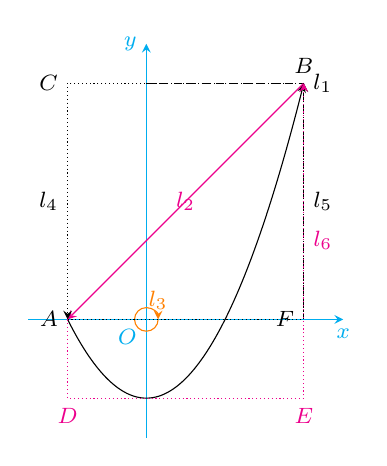
\begin{tikzpicture}[->,samples=100,>=stealth,font=\footnotesize]
                \draw[->,cyan](-1.5,0)--(0,0)node[below left]{$O$}--(2.5,0)node[below]{$x$};
                \draw[->,cyan](0,-1.5)--(0,3.5)node[left]{$y$};
                \draw[domain=-1:2,black] plot(\x,{\x*\x-1})node[right]{$l_1$};
                \node[below,left] at (-1,0) {$A$};
                \draw[densely dashed,-,black] (0,3)--(2,3)node[above]{$B$}--(2,0);
                \draw[magenta] (2,3)--(-1,0) node[midway]{$l_2$};
                \draw[orange] (0.15,0) arc (360:0:0.15) node[above]{$l_3$};
                \draw[densely dotted] (2,3)--(-1,3)node[left]{$C$}--(-1,0)node[midway,left]{$l_4$};
                \draw[densely dotted] (-1,0)--(2,0)node[below,left]{$F$}--(2,3)node[midway,right]{$l_5$};
                \draw[densely dotted,magenta] (-1,0)--(-1,-1)node[below]{$D$}--(0,-1)--(2,-1)node[below]{$E$}--(2,3)node[midway,right]{$l_6$};
            \end{tikzpicture}
            \caption{}
        \end{figure}
    \end{minipage}
    \textbf{法三: }$\displaystyle I=\int_{\stackrel\frown{AB}}\dfrac{-y}{x^2+y^2}\dd x+\dfrac{x}{x^2+y^2}\dd y=\int_{(-1,0^-)}^{(2,3)}\dd \qty(\arctan\dfrac{y}{x})=\int_{-\pi}^{\arctan\frac{3}{2}}\dd \theta=\arctan\dfrac{3}{2}+\pi.$\\
\end{solution}

\begin{example}
    已知 $\varphi(0)=\dfrac{1}{2}$,求连续可微函数 $\varphi(x)$,使得曲线积分 $\displaystyle\int_{A}^{B}\qty[\e^x+\varphi(x)]y\dd x-\varphi(x)\dd y$ 与路径无关.
\end{example}
\begin{solution}
    令 $P=\qty[\e^x+\varphi(x)]y,~Q=-\varphi(x)$,因为积分与路径无关,则 $$\pdv{P}{y}=\pdv{Q}{x}\Rightarrow \varphi'(x)+\varphi(x)=-\e^x$$
    该方程为一阶线性微分方程,有通解公式 $$\varphi(x)=\e^{-\int\dd x}\qty[\int\qty(-\e^{x})\cdot\e^{\int\dd x}\dd x+C]=-\dfrac{1}{2}\e^{x}+C\e^{-x}$$
    又因为 $\varphi(0)=\dfrac{1}{2}$,解得 $C=1$,因此 $\varphi(x)=-\dfrac{1}{2}\e^x+\e^{-x}.$
\end{solution}

\subsubsection{二重积分分部积分}

\begin{theorem}[二重积分分部积分公式]
    设 $D$ 是由一条或几条按段光滑的封闭曲线围成的平面有界闭区域,若函数  $u,v$ 在闭区域 $D$ 上有连续的一阶偏导数,则
    \label{iintlimitsduvxxy}
    $$\iint\limits _{D}u\dfrac{\partial v}{\partial x}\dd x\dd y=\oint _{\partial D}uv\dd y-\iint\limits _{D}v\dfrac{\partial u}{\partial x}\dd x\dd y,~\iint\limits _{D}u\dfrac{\partial v}{dy}\dd x\dd y=-\oint _{\partial D}uv\dd x-\iint\limits _{D}v\dfrac{\partial u}{\partial y}\dd x\dd y.$$
    \index{二重积分分部积分公式}
\end{theorem}

\begin{example}[2023 西北大学]
    设 $D$ 是由简单光滑闭曲线 $L$ 围成的区域,$f(x,y)$ 在 $D$ 上具有连续的偏导数,记作: $d=\max\limits_{(x,y)\in D}\sqrt{x^2+y^2}$,
    \begin{enumerate}[label=(\arabic{*})]
        \item 证明: $\displaystyle \iint\limits_D f(x,y)\dd x\dd y=\int_L x\cdot f \dd y-\iint\limits_Dx\pdv{f}{x}\dd x\dd y$;
        \item 若 $\forall (x,y)\in L$,有 $f(x,y)=0$,证明:
              $$\iint\limits_D f^2(x,y)\dd x\dd y\leqslant d^2\iint\limits_D\qty[\qty(\pdv{f}{x})^2+\qty(\pdv{f}{y})^2]\dd x\dd y.$$
    \end{enumerate}
\end{example}
\begin{proof}[{\songti \textbf{证}}]
    \begin{enumerate}[label=(\arabic{*})]
        \item 有 Green 公式得 $$\iint\limits_Du\pdv{v}{x}\dd x\dd y=\oint_{\partial D}uv\dd y-\iint\limits_Dv\pdv{u}{x}\dd x\dd y$$
              令 $u=x,~v=f$,则有 $\displaystyle\iint\limits_Dx\pdv{f}{x}\dd x\dd y=\int_Lx\cdot f\dd y-\iint\limits_Df(x,y)\dd x\dd y$,整理得证;
        \item 由 (1) 可得,$\displaystyle \iint\limits_D f^2\dd x\dd y=\dfrac{1}{2}\int_L f^2(x\dd y-y\dd x)-\dfrac{1}{2}\iint\limits_D\qty(x\pdv{f^2}{x}+y\pdv{f^2}{y})\dd x\dd y$
              又 $\forall (x,y)\in L$,有 $f(x,y)=0$,于是 $\displaystyle \int_Lf^2(x\dd y-y\dd x)=0$,故 $\displaystyle \iint\limits_D f^2\dd x\dd y=-\dfrac{1}{2}\iint\limits_D\qty(x\pdv{f^2}{x}+y\pdv{f^2}{y})\dd x\dd y$,
              于是由 Cauchy-Schwarz 不等式得,
              \begin{flalign*}
                  \iint\limits_D f^2\dd x\dd y & \leqslant \iint\limits_D\qty|xf\pdv{f}{x}+yf\pdv{f}{y}|\dd x\dd y\leqslant \iint\limits_D|f|\sqrt{x^2+y^2}\cdot\sqrt{\qty(\pdv{f}{x})^2+\qty(\pdv{f}{y})^2}\dd x\dd y                                                 \\
                                               & \leqslant d \iint\limits_D|f|\sqrt{\qty(\pdv{f}{x})^2+\qty(\pdv{f}{y})^2}\dd x\dd y\leqslant d\qty[\iint\limits_Df^2\dd x\dd y\cdot\iint\limits_D\qty(\qty(\pdv{f}{x})^2+\qty(\pdv{f}{y})^2)\dd x\dd y]^{\frac{1}{2}}
              \end{flalign*}
              即 $\displaystyle \qty(\iint\limits_Df^2\dd x\dd y)^{\frac{1}{2}}\leqslant d\cdot\qty[\iint\limits_D \qty(\qty(\pdv{f}{x})^2+\qty(\pdv{f}{y})^2)\dd x\dd y]^{\frac{1}{2}}$,不等式两边平方,即得证.
    \end{enumerate}
\end{proof}

\begin{example}
    设函数 $f(x,y)$ 在区域 $D:x^2+y^2\leqslant  1$ 上有二阶连续偏导数,
    且 $\displaystyle\frac{\partial^2f}{\partial x^2}+\frac{\partial^2f}{\partial y^2}=\mathrm{e}^{-\left(x^2+y^2\right)}$,证明:
    $$\iint\limits_D\left(x\frac{\partial f}{\partial x}+y\frac{\partial f}{\partial y}\right)\dd x\dd y=\frac{\pi}{2\mathrm{e}}.$$
\end{example}
\begin{proof}[{\songti \textbf{证法一}}]
    积分区域 $D$ 是圆形域,考虑采用极坐标,然后利用已知等式化简被积函数.
    令 $x=\rho\cos\theta,~y=\rho\sin\theta$,则$$D=\{(\rho,\theta)|0\leqslant \rho\le1,0\leqslant \theta\le2\pi\}$$ 于是
    $$\iint\limits_D\left(x\frac{\partial f}{\partial x}+y\frac{\partial f}{\partial y}\right)\dd x\dd y=\int_0^1\rho\dd \rho\int_0^{2\pi}\left(\rho\cos\theta\frac{\partial f}{\partial x}+\rho\sin\theta\frac{\partial f}{\partial y}\right)\dd \theta.$$
    记 $L_\rho$ 为半径是 $\rho\left(0\leqslant \rho\leqslant  1\right)$ 的圆周 (逆时针方向),$D_\rho$ 为 $L_\rho$ 包围的区域,则
    $$\int_0^{2\pi}\left(\rho\cos\theta\frac{\partial f}{\partial x}+\rho\sin\theta\frac{\partial f}{\partial y}\right)\dd \theta=\oint_{L_\rho}-\frac{\partial f}{\partial y}\dd x+\frac{\partial f}{\partial x}\dd y.$$
    由 Green 公式及已知等式,得
    $$\text{上式}=\iint\limits_{D_\rho}\left(\frac{\partial^2f}{\partial x^2}+\frac{\partial ^2f}{\partial y^2}\right)\dd x\dd y=\iint_{D_\rho}\mathrm{e}^{-\left(x^2+y^2\right)}\dd x\dd y=\int_0^{2\pi}\dd \theta\int_0^\rho\mathrm{e}^{-r^2}r\dd r=\pi\left(1-\mathrm{e}^{-\rho^2}\right)$$
    故 $$\iint\limits_D\left(x\frac{\partial f}{\partial x}+y\frac{\partial f}{\partial y}\right)\dd x\dd y=\int_0^1\rho\pi\left(1-\mathrm{e}^{-\rho^2}\right)\dd \rho=\frac{\pi}{2\mathrm{e}}.$$
\end{proof}
\begin{proof}[{\songti \textbf{证法二}}]
    由 Green 公式,可导出二重积分的分部积分公式:
    $$\iint\limits_Du\frac{\partial v}{\partial x}\dd x\dd y=\oint_{\partial D}uv\dd y-\iint\limits_Dv\frac{\partial u}{\partial x}\dd x\dd y,~\iint\limits_Du\frac{\partial v}{\partial y}\dd x\dd y=-\oint_{\partial D}uv\dd x-\iint\limits_Dv\frac{\partial u}{\partial y}\dd x\dd y.$$
    其中 $D$ 是由一条分段光滑闭曲线所围成的闭区域,$\partial D$ 为 $D$ 的正向边界.\\
    令 $\displaystyle u=\frac{\partial f}{\partial x},~\frac{\partial v}{\partial x}=x=\frac{\partial }{\partial x}\left(\frac{x^2+y^2}{2}\right)$,则由上述公式,有
    \begin{flalign*}
        \iint\limits_Dx\frac{\partial f}{\partial x}\dd x\dd y  =\iint\limits_D\frac{\partial f}{\partial x}\cdot\frac{\partial }{\partial x}\left(\frac{x^2+y^2}{2}\right)\dd x\dd y
        =\frac{1}{2}\oint_{\partial D}\left(x^2+y^2\right)\frac{\partial f}{\partial x}\dd y-\frac{1}{2}\iint\limits_D\left(x^2+y^2\right)\frac{\partial^2f}{\partial x^2}\dd x\dd y
    \end{flalign*}
    再令 $\displaystyle u=\frac{\partial f}{\partial y},~\frac{\partial v}{\partial x}=y=\frac{\partial }{\partial y}\left(\frac{x^2+y^2}{2}\right)$,类似地,有
    \begin{flalign*}
        \iint\limits_Dy\frac{\partial f}{\partial y}\dd x\dd y  =\iint\limits_D\frac{\partial f}{\partial y}\cdot\frac{\partial }{\partial y}\left(\frac{x^2+y^2}{2}\right)\dd x\dd y
        =-\frac{1}{2}\oint_{\partial D}\left(x^2+y^2\right)\frac{\partial f}{\partial y}\dd x-\frac{1}{2}\iint\limits_D\left(x^2+y^2\right)\frac{\partial ^2f}{\partial y^2}\dd x\dd y
    \end{flalign*}
    于是
    \begin{flalign*}
        \iint\limits_D\left(x\frac{\partial f}{\partial x}+y\frac{\partial f}{\partial y}\right)\dd x\dd y  =\frac{1}{2}\oint_{\partial D}\left(x^2+y^2\right)\frac{\partial f}{\partial x}\dd y-\left(x^2+y^2\right)\frac{\partial f}{\partial y}\dd x
        -\frac{1}{2}\iint\limits_D\left(x^2+y^2\right)\left(\frac{\partial ^2f}{\partial x^2}+\frac{\partial^2f}{\partial y^2}\right)\dd x\dd y.
    \end{flalign*}
    因为在边界 $\partial D$ 上,$x^2+y^2=1$,所以利用 Green 公式,得
    \begin{flalign*}
        \text{上式} & =\frac{1}{2}\oint_{\partial D}\frac{\partial f}{\partial x}\dd y-\frac{\partial f}{\partial y}\dd x-\frac{1}{2}\iint\limits_D\left(x^2+y^2\right)\mathrm{e}^{-\left(x^2+y^2\right)}\dd x\dd y                \\
                    & =\frac{1}{2}\iint\limits_D\left(\frac{\partial^2f}{\partial x^2}+\frac{\partial^2f}{\partial y^2}\right)\dd x\dd y-\frac{1}{2}\iint\limits_D\left(x^2+y^2\right)\mathrm{e}^{-\left(x^2+y^2\right)}\dd x\dd y \\
                    & =\frac{1}{2}\iint\limits_D\left(1-x^2-y^2\right)\mathrm{e}^{-\left(x^2+y^2\right)}\dd x\dd y
        =\frac{1}{2}\int_0^{2\pi}\dd \theta\int_0^1\left(1-\rho^2\right)\rho\mathrm{e}^{-\rho^2}\dd \rho=\frac{\pi}{2\mathrm{e}}.
    \end{flalign*}
\end{proof}

\begin{example}[首届数学竞赛数学类决赛]
    设 $f(x,y)$ 是 $D=\{(x,y)|x^2+y^2\leqslant  1\}$ 上二次连续可微函数,满足 $\displaystyle\frac{\partial^2f}{\partial x^2}+\frac{\partial^2f}{\partial y^2}=x^2y^2$,
    计算积分
    $$I=\iint\limits_D\left(\frac{x}{\sqrt{x^2+y^2}}\frac{\partial f}{\partial x}+\frac{y}{\sqrt{x^2+y^2}}\frac{\partial f}{\partial y}\right)\dd x\dd y.$$
\end{example}
\begin{solution}
    由 Green 公式,可导出二重积分的分部积分公式:
    $$\iint\limits_Du\frac{\partial v}{\partial x}\dd x\dd y=\oint_{\partial D}uv\dd y-\iint\limits_Dv\frac{\partial u}{\partial x}\dd x\dd y,~\iint\limits_Du\frac{\partial v}{\partial y}\dd x\dd y=-\oint_{\partial D}uv\dd x-\iint\limits_Dv\frac{\partial u}{\partial y}\dd x\dd y.$$
    其中 $D$ 是由一条分段光滑闭曲线所围成的闭区域,$\partial D$ 为 $D$ 的正向边界.\\
    令 $\displaystyle u=\frac{\partial f}{\partial x},~\frac{\partial v}{\partial x}=\frac{x}{\sqrt{x^2+y^2}}=\frac{\partial \sqrt{x^2+y^2}}{\partial x}$,则由上述公式,有
    \begin{flalign*}
        \iint\limits_Du\frac{\partial v}{\partial x}\dd x\dd y  =\iint\limits_D\frac{x}{\sqrt{x^2+y^2}}\frac{\partial f}{\partial x}\dd x\dd y
        =\oint_{\partial D}\sqrt{x^2+y^2}\frac{\partial f}{\partial x}\dd y-\iint\limits_D\sqrt{x^2+y^2}\frac{\partial^2f}{\partial x^2}\dd x\dd y
    \end{flalign*}
    再令 $\displaystyle u=\frac{\partial f}{\partial y},~\frac{\partial v}{\partial y}=\frac{y}{\sqrt{x^2+y^2}}=\frac{\partial \sqrt{x^2+y^2}}{y}$,类似地,有
    \begin{flalign*}
        \iint\limits_Du\frac{\partial v}{\partial y}\dd x\dd y =\iint\limits_D\frac{y}{\sqrt{x^2+y^2}}\frac{\partial f}{\partial y}\dd x\dd y
        =-\oint_{\partial D}\sqrt{x^2+y^2}\frac{\partial f}{\partial y}\dd x-\iint\limits_D\sqrt{x^2+y^2}\frac{\partial^2f}{\partial x^2}\dd x\dd y
    \end{flalign*}
    于是
    \begin{flalign*}
        \iint\limits_D\left(\frac{x}{\sqrt{x^2+y^2}}\frac{\partial f}{\partial x}+\frac{y}{\sqrt{x^2+y^2}}\frac{\partial f}{\partial y}\right)\dd x\dd y & =\oint_{\partial D}\sqrt{x^2+y^2}\frac{\partial f}{\partial x}\dd y-\sqrt{x^2+y^2}\frac{\partial f}{\partial y}\dd x\dd y \\
                                                                                                                                                         & ~ -\iint\limits_D\sqrt{x^2+y^2}\left(\frac{\partial^2f}{\partial x^2}+\frac{\partial^2f}{\partial y^2}\right)\dd x\dd y
    \end{flalign*}
    因为在边界 $\partial D$ 上,$x^2+y^2=1$,所以利用 Green 公式,得
    \begin{flalign*}
        \text{上式} & =\oint_{\partial D}\frac{\partial f}{\partial x}\dd y-\frac{\partial f}{\partial y}\dd x-\iint\limits_D\sqrt{x^2+y^2}\cdot x^2y^2\dd x\dd y
        =\iint\limits_D\left(\frac{\partial^2f}{\partial x^2}+\frac{\partial^2f}{\partial y^2}\right)\dd x\dd y-\iint\limits_Dx^2y^2\sqrt{x^2+y^2}\dd x\dd y      \\
                    & =\iint\limits_Dx^2y^2\left(1-\sqrt{x^2+y^2}\right)\dd x\dd y
        =\int_0^{2\pi}\cos^2\theta\sin^2\theta\dd \theta\int_0^1\rho^5(1-\rho)\dd \rho=\frac{\pi}{168}
    \end{flalign*}
\end{solution}

\begin{example}[第十三届数学竞赛非数学预赛补赛]
    设函数 $f(x,y)$ 在闭区间 $D=\{(x,y)|x^2+y^2\leqslant  1\}$ 上具有二阶连续偏导数,
    且 $\displaystyle\frac{\partial^2f}{\partial x^2}+\frac{\partial^2f}{\partial y^2}=x^2+y^2$,
    求 $$\displaystyle\lim_{r\to0^+}\frac{\displaystyle\iint\limits_{x^2+y^2\leqslant  r^2}\left(x\frac{\partial f}{\partial x}+y\frac{\partial f}{\partial y}\right)\dd x\dd y}{\left(\tan r-\sin r\right)^2}.$$
\end{example}
\begin{solution}
    记 $D_r=x^2+y^2\leqslant  r^2$,由 Green 公式,可导出二重积分的分部积分公式:
    $$\iint\limits_{D_r}u\frac{\partial v}{\partial x}\dd x\dd y=\oint_{\partial D_r}uv\dd y-\iint\limits_{D_r}v\frac{\partial u}{\partial x}\dd x\dd y,~\iint\limits_{D_r}u\frac{\partial v}{\partial y}\dd x\dd y=-\oint_{\partial D_r}uv\dd x-\iint\limits_{D_r}v\frac{\partial u}{\partial y}\dd x\dd y.$$
    其中 $D_r$ 是由一条分段光滑闭曲线所围成的闭区域,$\partial D_r$ 为 $D_r$ 的正向边界.\\
    令 $\displaystyle u=\frac{\partial f}{\partial x},~\frac{\partial v}{\partial x}=x=\frac{\partial }{\partial x}\left(\frac{x^2+y^2}{2}\right)$,则由上述公式,有
    \begin{flalign*}
        \iint\limits_{D_r}x\frac{\partial f}{\partial x}\dd x\dd y =\iint\limits_{D_r}\frac{\partial f}{\partial x}\cdot\frac{\partial }{\partial x}\left(\frac{x^2+y^2}{2}\right)\dd x\dd y
        =\frac{1}{2}\oint_{\partial D_r}\left(x^2+y^2\right)\frac{\partial f}{\partial x}\dd y-\frac{1}{2}\iint\limits_{D_r}\left(x^2+y^2\right)\frac{\partial^2f}{\partial x^2}\dd x\dd y
    \end{flalign*}
    再令 $\displaystyle u=\frac{\partial f}{\partial y},~\frac{\partial v}{\partial y}=y=\frac{\partial}{\partial y}\left(\frac{x^2+y^2}{2}\right)$,类似地,有
    \begin{flalign*}
        \iint\limits_{D_r}y\frac{\partial f}{\partial y}\dd x\dd y =\iint\limits_{D_r}\frac{\partial f}{\partial y}\cdot\frac{\partial }{\partial y}\left(\frac{x^2+y^2}{2}\right)\dd x\dd y
        =-\frac{1}{2}\oint_{\partial D_r}\left(x^2+y^2\right)\frac{\partial f}{\partial y}\dd x-\frac{1}{2}\iint\limits_{D_r}\left(x^2+y^2\right)\frac{\partial^2f}{\partial y^2}\dd x\dd y
    \end{flalign*}
    于是
    \begin{flalign*}
        \iint\limits_{D_r}\left(x\frac{\partial f}{\partial x}+y\frac{\partial f}{\partial y}\right)\dd x\dd y =\frac{1}{2}\oint_{\partial D_r}\left(x^2+y^2\right)\frac{\partial f}{\partial x}\dd y-\left(x^2+y^2\right)\frac{\partial f}{\partial y}\dd x
        -\frac{1}{2}\iint\limits_{D_r}\left(x^2+y^2\right)\left(\frac{\partial^2f}{\partial x^2}+\frac{\partial^2f}{\partial y^2}\right)\dd x\dd y
    \end{flalign*}
    因为在边界 $\partial D_r$ 上,$x^2+y^2=r^2$,所以利用 Green 公式,得
    \begin{flalign*}
        \text{上式} & =\frac{r^2}{2}\oint_{\partial D_r}\frac{\partial f}{\partial x}\dd y-\frac{\partial f}{\partial y}\dd x-\frac{1}{2}\iint\limits_{D_r}\left(x^2+y^2\right)^2\dd x\dd y
        =\frac{r^2}{2}\iint\limits_{D_r}\left(x^2+y^2\right)\dd x\dd y-\frac{1}{2}\iint\limits_{D_r}\left(x^2+y^2\right)^2\dd x\dd y                                                        \\
                    & =\frac{1}{2}\iint\limits_{D_r}\left[r^2\left(x^2+y^2\right)-\left(x^2+y^2\right)^2\right]\dd x\dd y
        =\frac{1}{2}\int_0^{2\pi}\dd \theta\int_0^r\left(r^2\rho^3-\rho^5\right)\dd \rho=\frac{\pi r^6}{12}
    \end{flalign*}
    另一方面,$\displaystyle\left(\tan r-\sin r\right)^2=\left(r+\frac{r^3}{3}-r+\frac{r^3}{6}+o\left(r^3\right)\right)^2\sim\frac{r^6}{4},~r\to0^+.$\\
    综上,原式=$\displaystyle\lim_{r\to0^+}\frac{\pi r^6}{12}\cdot\frac{4}{r^6}=\frac{\pi}{3}$.
\end{solution}

\begin{example}
    设 $u(x,y)$ 在 $D:x^2+y^2\leqslant 1$ 上有二阶连续偏导数,且 $\displaystyle\pdv[2]{u}{x}+\pdv[2]{u}{y}=\dfrac{x^2+y^2}{\e^{x}+\e^{y}}\cdot\e^{x}$,
    试求 $$\displaystyle\lim_{t\to0^+}\dfrac{\displaystyle\iint\limits_{x^2+y^2\leqslant t^2}\qty(x\cdot\pdv{u}{x}+y\cdot\pdv{u}{y})\dd x\dd y}{(\tan t-\arctan t)^2}.$$
\end{example}
\begin{solution}
    令 $D_t:x^2+y^2\leqslant t^2$,由 Green 公式可得二重积分分部积分公式,
    $$\begin{cases}
            \displaystyle \iint\limits_{D_t}x\pdv{u}{x}\dd x\dd y=\oint_{\partial D_t}\pdv{u}{x}\cdot\dfrac{x^2+y^2}{2}\dd y-\iint\limits_{D_t}\dfrac{x^2+y^2}{2}\cdot\pdv[2]{u}{x}\dd x\dd y \\
            \displaystyle \iint\limits_{D_t}y\pdv{u}{y}\dd x\dd y=-\oint_{\partial D_t}\pdv{u}{y}\cdot\dfrac{x^2+y^2}{2}\dd x-\iint\limits_{D_t}\dfrac{x^2+y^2}{2}\cdot\pdv[2]{u}{y}\dd x\dd y
        \end{cases}$$
    于是
    \begin{flalign*}
        I & =\iint\limits_{D_t}\qty(x\cdot\pdv{u}{x}+y\cdot\pdv{u}{y})\dd x\dd y=\dfrac{t^2}{2}\oint_{\partial D_t}\pdv{u}{x}\dd y-\pdv{u}{y}\dd x-\dfrac{1}{2}\iint\limits_{D_t}\qty(x^2+y^2)\qty(\pdv[2]{u}{x}+\pdv[2]{u}{y})\dd x\dd y \\
          & =\dfrac{1}{2}\iint\limits_{D_t}\qty[t^2-\qty(x^2+y^2)]\qty(\pdv[2]{u}{x}+\pdv[2]{u}{y})\dd x\dd y=\dfrac{1}{2}\iint\limits_{D_t}\qty[t^2-\qty(x^2+y^2)]\qty(x^2+y^2)\cdot\dfrac{\e^{x}}{\e^{x}+\e^{y}}\dd x\dd y              \\
          & =\dfrac{\e^{\xi}}{2\qty(\e^{\xi}+\e^{\eta})}\int_{0}^{2\pi}\dd \theta\int_{0}^{t}\qty[t^2-r^2]r^3\dd r=\dfrac{\e^{\xi}}{2\qty(\e^{\xi}+\e^{\eta})}\cdot2\pi\cdot\dfrac{t^6}{12}
    \end{flalign*}
    其中 $(\xi,\eta)\in D_t$,那么
    \begin{flalign*}
        \lim_{t\to0^+}\dfrac{\displaystyle\iint\limits_{x^2+y^2\leqslant t^2}\qty(x\cdot\pdv{u}{x}+y\cdot\pdv{u}{y})\dd x\dd y}{(\tan t-\arctan t)^2}=\lim_{t\to0^+}\dfrac{\dfrac{\e^{\xi}\pi t^6}{12\qty(\e^{\xi}+\e^{\eta})}}{\qty(-\dfrac{2}{3}t^3)^2}=\dfrac{3\pi}{32}.
    \end{flalign*}
\end{solution}

\begin{example}[第九届数学竞赛决赛]
    设函数 $f(x,y)$ 在区域 $D=\left\{(x,y)|x^2+y^2\leqslant  a^2\right\}$ 上是有一阶连续偏导数,
    且满足 $$f(x,y)|_{x^2+y^2=a^2}=a^2\text{,以及} \displaystyle\max\limits_{(x,y)\in D}\left[\left(\frac{\partial f}{\partial x}\right)^2+\left(\frac{\partial f}{\partial y}\right)^2\right]=a^2$$
    其中 $a>0$. 证明: $\displaystyle\left |\iint\limits_Df(x,y)\dd x\dd y\right |\leqslant \frac{4}{3}\pi a^4$.
\end{example}
\begin{proof}[{\songti \textbf{证}}]
    由 Green 公式,可导出二重积分的分部积分公式:
    $$\iint\limits_Du\frac{\partial v}{\partial x}\dd x\dd y=\oint_{\partial D}uv\dd y-\iint\limits_Dv\frac{\partial u}{\partial x}\dd x\dd y,~\iint\limits_Du\frac{\partial v}{\partial y}\dd x\dd y=-\oint_{\partial D}uv\dd x-\iint\limits_Dv\frac{\partial u}{\partial y}\dd x\dd y.$$
    其中 $D$ 是由一条分段光滑闭曲线所围成的闭区域,$\partial D$ 为 $D$ 的正向边界.\\
    令 $\displaystyle\frac{\partial v}{\partial x}=1=\frac{\partial x}{\partial x},~u=f(x,y)$ ,则由上述公式,有
    \begin{flalign*}
        \iint\limits_Du\frac{\partial v}{\partial x}\dd x\dd y=\iint\limits_Df(x,y)\dd x\dd y=\oint_{\partial D}xf(x,y)\dd y-\iint\limits_Dx\frac{\partial f}{\partial x}\dd x\dd y
    \end{flalign*}
    再令 $\displaystyle\frac{\partial v}{\partial y}=1=\frac{\partial y}{\partial y},~u=f(x,y)$,则有
    \begin{flalign*}
        \iint\limits_Du\frac{\partial v}{\partial y}\dd x\dd y=\iint\limits_Df(x,y)\dd x\dd y=-\oint_{\partial D}yf(x,y)\dd x-\iint\limits_Dy\frac{\partial f}{\partial y}\dd x\dd y
    \end{flalign*}
    所以由 Cauchy-Schwarz 不等式,
    \begin{flalign*}
        \left |\iint\limits_Df(x,y)\dd x\dd y\right | & =\frac{1}{2}\oint_{\partial D}\left |xf(x,y)\dd y-yf(x,y)\dd x\right |+\frac{1}{2}\iint\limits_D\left |x\frac{\partial f}{\partial x}+y\frac{\partial f}{\partial y}\right |\dd x\dd y   \\
                                                      & \leqslant  a^2\iint\limits_D\dd x\dd y+\frac{1}{2}\iint\limits_D\sqrt{x^2+y^2}\sqrt{\left(\frac{\partial f}{\partial x}\right)^2+\left(\frac{\partial f}{\partial y}\right)^2}\dd x\dd y \\
                                                      & \leqslant  \pi a^4+\frac{a}{2}\iint\limits_D\sqrt{x^2+y^2}\dd x\dd y
        =\pi a^4+\int_0^{2\pi} \dd \theta\int_0^a\rho^2\dd \rho=\frac{4}{3}\pi a^4
    \end{flalign*}
\end{proof}
